\documentclass{beamer}
\usepackage[utf8]{inputenc}
\usetheme{Madrid}
\usecolortheme{default}
\usepackage{amsmath,amssymb,amsfonts,amsthm}
\usepackage{mathtools}
\usepackage{txfonts}
\usepackage{tkz-euclide}
\usepackage{listings}
\usepackage{adjustbox}
\usepackage{array}
\usepackage{tabularx}
\usepackage{gvv}
\usepackage{lmodern}
\usepackage{circuitikz}
\usepackage{tikz}
\usepackage{graphicx}
\setbeamertemplate{page number in head/foot}[totalframenumber]
\usepackage[T1]{fontenc}
\usepackage{tcolorbox}
\tcbuselibrary{minted,breakable,xparse,skins}

\definecolor{bg}{gray}{0.95}
\DeclareTCBListing{mintedbox}{O{}m!O{}}{%
  breakable=true,
  listing engine=minted,
  listing only,
  minted language=#2,
  minted style=default,
  minted options={%
    linenos,
    gobble=0,
    breaklines=true,
    breakafter=,,
    fontsize=\small,
    numbersep=8pt,
    #1},
  boxsep=0pt,
  left skip=0pt,
  right skip=0pt,
  left=25pt,
  right=0pt,
  top=3pt,
  bottom=3pt,
  arc=5pt,
  leftrule=0pt,
  rightrule=0pt,
  bottomrule=2pt,
  toprule=2pt,
  colback=bg,
  colframe=orange!70,
  enhanced,
  overlay={%
    \begin{tcbclipinterior}
    \fill[orange!20!white] (frame.south west) rectangle ([xshift=20pt]frame.north west);
    \end{tcbclipinterior}},
  #3,
}

% Code style
\lstset{
    language=C,
    basicstyle=\ttfamily\small,
    keywordstyle=\color{blue},
    stringstyle=\color{orange},
    commentstyle=\color{green!60!black},
    numbers=left,
    numberstyle=\tiny\color{gray},
    breaklines=true,
    showstringspaces=false,
}

% Title info
\title %optional
{5.8.16}
\date{October 9, 2025}
\author % (optional)
{EE25BTECH11018 - Darisy Sreetej}

\begin{document}

\frame{\titlepage}

\begin{frame}{Question}
The taxi charges in a city consist of a fixed charge together with the charges for the distance covered. For a distance of 10 km, the charge paid is Rs.105 and for a distance of 15 km, the charge paid is Rs.155. What are the fixed charges and the charge per km? How much does a person have to pay for travelling a distance of 25 km ?
\end{frame}
\begin{frame}{Solution}
Let us solve the given question theoretically and then verify the solution computationally.\\
Let
x = fixed charge , 
y = charge per km \\
Then total fare = $x + y \times distance$\\
According to the question,
The equation of lines given
\begin{align}
    \myvec{1&&10}\vec{x}=105 \\
    \myvec{1&&15}\vec{x}=115 
    \end{align}
    where ,\quad $\vec{x}=\myvec{x\\y}$
\end{frame}
\begin{frame}
    From the question ,
\begin{align}
     \myvec{1&&25}\vec{x}=c 
     \end{align}
      where ,\quad $c$ = total fare the person should pay for travelling 25 km
\begin{align}
    \therefore \myvec{1&&10\\1&&15\\1&&25}\vec{x}=\myvec{105\\155\\c}
\end{align}
Using augmented matrix,
\begin{align}
    \augvec{2}{1}{1&10&105\\1&15&155\\1&25&c}
\end{align}
\end{frame}
\begin{frame}
    Upon doing row reduction,
\begin{align}
\begin{aligned}
       \augvec{2}{1}{1&10&105\\1&15&155\\1&25&c}
     \xleftrightarrow{R_3 = R_3 - R_1}
       \augvec{2}{1}{1&10&105\\1&15&155\\0&15&c-105}
\end{aligned}
\end{align}
\begin{align}
\begin{aligned}
      \augvec{2}{1}{1&10&105\\1&15&155\\0&15&c-105}
     \xleftrightarrow{R_2 = R_2 - R_1}
       \augvec{2}{1}{1&10&105\\0&5&50\\0&15&c-105}
\end{aligned}
\end{align}
\begin{align}
\begin{aligned}
      \augvec{2}{1}{1&10&105\\0&5&50\\0&15&c-105}
     \xleftrightarrow{R_3 = R_3 - 3 \times R_2}
     \augvec{2}{1}{1&10&105\\0&5&50\\0&0&c-255}
\end{aligned}
\end{align}
\end{frame}
\begin{frame}
    From (0.8),
\begin{align}
    \begin{aligned}
        0=c-255\\
        c=255\\
    \end{aligned}
\end{align}
\begin{align}
    \begin{aligned}
       5y=50\\
       y=10\\
       x+10y=105\\
       x=5
    \end{aligned}
\end{align}
\begin{align}
    \implies \vec{x}=\myvec{5\\10}
\end{align}
Thus , fixed charge =Rs.5\\
charge per km = Rs.10\\
The total fare the person should pay for travelling 25 km = Rs.255
\end{frame}
\begin{frame}{Plot}
    
 \begin{figure}[H]
     \centering
     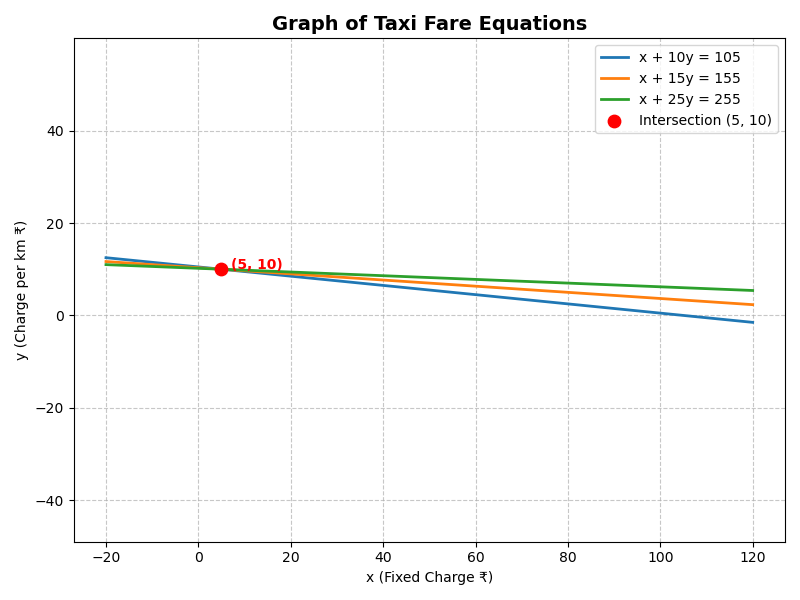
\includegraphics[width=0.8\columnwidth]{figs/fig.png}
     \label{fig:1}
 \end{figure}
\end{frame}
\begin{frame}[fragile]
\frametitle{C code}
    \begin{lstlisting}[language=C]
#include <stdio.h>

void solveByMatrix(float *x, float *y)
{
    float a[2][3] = {
        {1, 10, 105},
        {1, 15, 155}
    };

    float ratio;

    // Eliminate x from second row
    ratio = a[1][0] / a[0][0];
    for (int j = 0; j < 3; j++)
        a[1][j] = a[1][j] - ratio * a[0][j];

\end{lstlisting}
\end{frame}
\begin{frame}[fragile]
    \frametitle{C Code }
    \begin{lstlisting}[language=C]
         // Solve
    *y = a[1][2] / a[1][1];
    *x = (a[0][2] - a[0][1] * (*y)) / a[0][0];
}

     \end{lstlisting}
\end{frame}
\begin{frame}[fragile]
    \frametitle{Python + C code}

    \begin{lstlisting}[language=Python]
import ctypes
import numpy as np
import matplotlib.pyplot as plt

# --- Load shared library (.so) ---
lib = ctypes.CDLL("./taxi_matrix.so")

# Prepare C float variables
x = ctypes.c_float()
y = ctypes.c_float()

# Call the C function
lib.solveByMatrix(ctypes.byref(x), ctypes.byref(y))

# Extract computed values
x_val = x.value
y_val = y.value


    \end{lstlisting}
\end{frame}

\begin{frame}[fragile]
    \frametitle{Python + C code}

    \begin{lstlisting}[language=Python]
print(f"Fixed charge (x) = ₹{x_val:.2f}")
print(f"Charge per km (y) = ₹{y_val:.2f}")

# --- Generate data for plotting ---
x_vals = np.linspace(-20, 120, 400)

# Line equations from the problem
y1 = (105 - x_vals) / 10
y2 = (155 - x_vals) / 15
y3 = (255 - x_vals) / 25  # third line for c = 255

# Intersection point (from C)
x_int, y_int = x_val, y_val

# --- Plot configuration ---
plt.figure(figsize=(9, 6))
plt.style.use('seaborn-v0_8-whitegrid')
\end{lstlisting}
\end{frame}
\begin{frame}[fragile]
\frametitle{Python + C code}
    \begin{lstlisting}[language=Python]
        # Plot lines with clarity
plt.plot(x_vals, y1, color='royalblue', linewidth=2.8, label=r'$x + 10y = 105$')
plt.plot(x_vals, y2, color='darkorange', linewidth=2.8, linestyle='--', label=r'$x + 15y = 155$')
plt.plot(x_vals, y3, color='green', linewidth=2.8, linestyle='-.', label=r'$x + 25y = 255$')


# Intersection point
plt.scatter(x_int, y_int, color='red', s=100, edgecolors='black', zorder=5, label=f'Intersection ({x_int:.0f}, {y_int:.0f})')
plt.text(x_int + 5, y_int + 1, f'({x_int:.0f}, {y_int:.0f})', fontsize=12, color='red', fontweight='bold')
    \end{lstlisting}
\end{frame}
\begin{frame}[fragile]
\frametitle{Python + C code}
    \begin{lstlisting}[language=Python]
# --- Labels and aesthetics ---
plt.title("Graph of Taxi Fare Equations", fontsize=15, fontweight='bold')
plt.xlabel("x (Fixed Charge ₹)", fontsize=12)
plt.ylabel("y (Charge per km ₹)", fontsize=12)

plt.grid(True, linestyle='--', linewidth=0.7, alpha=0.8)
plt.legend(fontsize=11, loc='upper right', frameon=True, shadow=True)
plt.xlim(-20, 120)
plt.ylim(-50, 50)
plt.tight_layout()

plt.show()

     \end{lstlisting}
\end{frame}
\begin{frame}[fragile]
    \frametitle{Python code}
    \begin{lstlisting}[language=Python]
import numpy as np
import matplotlib.pyplot as plt

# Define y = (const - x)/coefficient equations
x_vals = np.linspace(-20, 120, 400)

# Line equations
y1 = (105 - x_vals) / 10
y2 = (155 - x_vals) / 15
y3 = (255 - x_vals) / 25  # c = 255

# Intersection point (x=5, y=10)
x_int, y_int = 5, 10

# Plot all lines
plt.figure(figsize=(8,6))
plt.plot(x_vals, y1, label="x + 10y = 105", linewidth=2)


    \end{lstlisting}
\end{frame}
\begin{frame}[fragile]
    \frametitle{Python code}
    \begin{lstlisting}[language=Python]
plt.plot(x_vals, y2, label="x + 15y = 155", linewidth=2)
plt.plot(x_vals, y3, label="x + 25y = 255", linewidth=2)
# Mark intersection
plt.scatter(x_int, y_int, color='red', s=80, zorder=5, label="Intersection (5, 10)")
# Annotate intersection
plt.text(x_int + 2, y_int, "(5, 10)", color='red', fontsize=10, fontweight='bold')
# Labels and title
plt.title("Graph of Taxi Fare Equations", fontsize=14, fontweight='bold')
plt.xlabel("x (Fixed Charge ₹)")
plt.ylabel("y (Charge per km ₹)")
plt.grid(True, linestyle="--", alpha=0.7)
plt.legend()
plt.axis("equal")  # to maintain aspect ratio
plt.tight_layout()
plt.show()
     \end{lstlisting}
\end{frame}
\end{document}
